

\section{Dynamisch programmierter Algorithmus \cite{dynamisch}}

\subsection{Herleitung}
Die Grundlage dieses Algorithmus ist der Robinson-Schensted Algorithmus, welcher in erster Linie sog. Young-Tableu berechnet. Das sind Darstellungen von Symmetriegruppen. In dem zugrunde liegenden Paper wird hauptsächlich aus dem Algorithmus eine Vereinfachung hergeleitet, welche das HIS Problem löst, jedoch gibt es anschauchlichere Herleitung, die den Algorithmus besser verdeutlicht.\\
Es handelt sich um einen dynamisch programmierten Algorithmus. Diese haben es an sich, oft zu betrachten, ob die Erweiterung einer bestehenden Lösung um ein Element, sich aus der $"$kleineren$"$ Lösung herleiten lässt, d.h. in dem Fall konkret, ob eine HIS einer Folge \an, auf eine HIS einer um 1 größeren Folge \an$a_{n+1}$ folgern lässt. Dabei wird eine Tabelle geführt, welche für einen Eintrag an der Stelle $i$ die HIS der (Teil-)Folge $a_1\dots a_i$ abspeichert, welche auf $a_i$ endet. Wenn man nun das $i+1$-te Element betrachtet, ergeben sich folgende drei Fälle:
\begin{enumerate}
    \item Die HIS der kleineren Folge bleibt die HIS der größeren Folge.
    \item Die HIS der kleineren Folge kann um das neue Element erweitert werden und ist danach die HIS der größeren Folge.
    \item Die HIS endet auf dem neuen Element, ist aber nicht die vorherige HIS erweitert.
\end{enumerate}
Interessant ist hierbei Fall 3, denn dafür müsste man andere mögliche Durchläufe speichern. In der Tabelle muss also mehr als ein Tupel ggf. sein, da aber insgesamt $n$ Elemente betrachtet werden, also nur eine Teilfolge, die auf einem $a_i$ endet, ist die Tabellengröße $n$. 
Mit dieser Anforderung können die drei Fälle erkannt werden, indem man die größte der erweiterbaren Folgen - also das größte Element kleiner dem Neuen, vgl. $prev$ aus Kapitel 2- mit dem Neuen erweitert, und ggf. Folgeelemente gelöscht werden. Da wir Paare als Elemente haben, und wir eine strikte Monotonie in beiden Elementen wollen (impliziert eine Sortierung, welche $prev$ schneller berechnen lässt), müssen wir ggf. größere Elemente in der ersten Koordinate löschen, die in der zweiten kleiner sind. Dazu eine kleine Erklärung:\\ 
\newtheorem{beispiel}{Beispiel}
\\
Man möchte das Element $(s,t)$ aus der Liste mit der neuen Zahl $a_i=:x$ erweitern und kriegt dann $(x,t+x)$. Alle Elemente $(u,v)$ mit $x \leq u$ kommen in der Liste danach. Jedoch kann man nicht beeinflussen, ob $v$ kleiner $t+x$ ist. Nehmen wir solch ein Element im Folgenden an. Wenn jetzt $(u,v)$ mit einem Element $a_j$ erweitert wird, muss $a_j$ größer als $u$ sein, demnach auch größer als $x$. Da aber auch $t+x$ größer als $v$ ist, ist auch $t+x+a_j$ größer als $v+a_j$. Dies gilt für alle Elemente die $u$ erweitern können, dadurch kann man alle $(u,v)$ mit $v$ kleiner $t+x$ löschen. Diese können nicht mehr die HIS werden, da jede Erweiterung von $(u,v)$ auch eine von $(x,t+x)$ darstellt.\\
Ein kleines Beispiel dazu ist die Folge $4,2,3,6$. Die Werte in der Liste sind bis zum Wert 3 $(2,2),(4,4)$ und danach die 3 eingefügt $(2,2),(3,5),(4,4)$. Für die 6 kommen sowohl $(3,5)$ als auch $(4,4)$ in Frage - $(2,2)$ auch, aber das hilft der Illustration nicht. 3 erweitert mit 6 ist größer, als 4 erweitert. Das liegt daran, dass die zweite Koordinate von $(3,5)$ größer als die in $(4,4)$ ist. Die Zahl 6 kann hier jede andere beliebige Zahl $x$ mit $x>4$ sein und die Aussage bleibt bestehen. Somit kann die $(4,4)$ gelöscht werden nachdem $(3,5)$ eingesetzt wurde, denn alles was $(4,4)$ erweitert, erweitert auch $(3,5)$.
\\
Nach diesem Prinzip ist die Listen in beiden Koordinaten streng monoton steigend. Wenn man also jetzt das letzte Element in der Liste herausnimmt, hat man das Element auf welches die HIS endet und die Summe der HIS.
\begin{beispiel}
    Sei $(a_n)=4;3;6;1;7;9;23$. Für das 5-te Element müssen alle Elemente in der Liste angeschaut werden, welche kleiner als $a_5=7$ sind, das sind 4,3,6 und 1. Die Abbildung unten beschreibt den Zustand der Liste bevor das Element $7$ eingefügt wurde und zeigt, wo es eingefügt werden muss und wie sich der neue Wert ergibt. Die Abbildung darunter beschreibt die Änderung, welche sich bei $a_3=4$ statt $6$ ergeben würde.
\end{beispiel}
\begin{center}
	\begin{tabular}{c}
		
		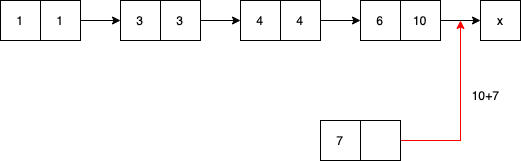
\includegraphics[scale=0.7]{./Pictures/pic2.png}\\
		\hline
		\includegraphics[scale=0.7]{./Pictures/löschen.png}\\
		
	\end{tabular}
\end{center}

\subsection{Algorithmus}
 
Wir wollen also aus der Herleitung der Idee jetzt einen konkreten Algorithmus formulieren. Sei im Folgenden \an eine Folge von natürlichen Zahlen. Als Ordnung und Gewicht nehmen wir die Werte der Zahlen selber. Der Algorithmus läuft dann wie folgt:
\begin{enumerate}
    \item Initialisiere eine leere Liste L und ein leeres Array $nodes$ der Länge $n$.
    \item Gehe nach und nach durch jedes Element $a_x$ in der Folge durch und mache Schritte 3 bis 5.
    \item Finde $(a,b)=prev(L,x)$ und $(c,d)=next(L,x)$.
    \item Solange $(c,d)$ existert und $d<b+x$ ist, führe $delete(L,(c,d))$ aus und setze $(c,d)=next(L,x)$.
    \item Füge $(x,b+x)$ ($(a,b)$ erweitert um x) in die L ein und setze $nodes[x]$ auf $a$.
\end{enumerate}

Das $nodes$-Array kann am Ende zur Rekonstruktion benutzt werden. Es ist auch eine leichte Vereinfachung des originalen Algorithmus vorhanden, da die Gewichtsfunktion hier nur vom Wert der Zahl abhängt und nicht auch noch von der Position. Als Pseudocode wäre das Ganze dann so: \newpage

\begin{lstlisting}[mathescape]
his($a_n$)
{
    %Step 1
    L=$ø$
    %step2
    for(i = 1; i <= n; i++)
    {
        %Step 3
        (s,v)=prev(L,($a_i$,0)) %Finds next smallest Element in List
        (t,w)=next(L,(s,v)) %Finds next largest Element in List

        %Step 4
        while((t,w) != $ø$)
        {
            if(v+$a_i$ < w)
                break;
            delete(L,(t,w))
            (t,w)=next(L,(t,w))
        }

        %Step 5
        if((t,w)$\neq\phi$||$a_i$<t)
       		 insert(L,($a_i$,v+$a_i$))
        nodes[$a_i$]= newnode($a_i$,node[s])
    }
}
\end{lstlisting}
\small Bemerkung:
\begin{quote}
    \footnotesize In Zeile 24 wird $nodes[a_i]$ auf ein $newnode$ Element gesetzt, dies dient zum Speichern der aktuellen Zahl, und an welcher Stelle in $nodes$ die vorherige Zahl in der HIS zu finden ist. Man kann also die HIS in umgekehrter Reihenfolge rekonstruieren. Diese Tabelle ist auch der Grund für das DP, die Liste dient als Hilfe zum Befüllen der Einträge.
\end{quote}
\normalsize


\subsection{Korrektheit}
Für die Korrektheit des Algorithmus' formulieren wir eine Invariante, die nach jeder Iteration des Algorithmus' gelten soll:\\
Sei $L$ die Liste für das Abspeichern der Tupel und $a_1 \dots a_n$ die Folge, für die die HIS gefunden werden soll. Nach der i-ten Iteration für die Zahl $a_i$ gilt: Für jede streng monotone Teilefolge $(b_k)$ in $a_1 \dots a_i$ gibt es ein Tupel $(s,t)$ in der Liste $L$ mit $s\leq b_i$ und $ t \geq \sum_{j=1}^k b_j$. Da für jede endliche Folge eine HIS $b_1 \dots b_k$ existiert, gilt dies auch für die HIS, das heißt, es gibt ein Element $(s,t)$ in L mit $s\leq b_k$ und $t\geq \sum_{j=1}^k b_j$. Wenn man dann aus $L$ das letzte Element (größte) herausnimmt, kriegt man die HIS.

\newtheorem{beweis}{Beweis}

\begin{beweis}
Wir beweisen die Invariante mit Induktion über die aktuelle Iteration im Algorithmus (i-te Iteration). Sei nun $L$ eine Datenstruktur, welche die geforderten Funktionalitäten erfüllt, und $a_1 \dots a_n$ eine Folge an Zahlen (Im Allgemeinen gilt dies auch für eine Menge mit Gewichtung und Ordnung). Für $i=1$ ergibt sich nur eine einzige Teilfolge, nämlich die Folge $a_1$ selber. Nach Zeile 24 im Algorithmus wird bei einem leeren L ein Element in die Liste eingefügt, in dem Fall $(a_i,a_i)$. Daraus folgt die Aussage für $i=1$.\\
Gelte also für ein festes aber beliebiges $i$ die Annahme. Man betrachte nun $a_1 \dots a_{i+1}$ für die $(i+1)$-te Iteration. Nach Annahme gibt für jede monotone Teilfolge $(b_k)$ aus $a_1 \dots a_{i}$ ein Tupel $(s,t)$ in der Liste, welches die Anforderung der Invariante erfüllt. Daraus ergeben sich drei Fälle: $a_{i+1}=b_k$, $a_{i+1}>b_k$ und $a_{i+1} < b_k$. Sei $(s,t)$ das Element aus L, welche für $(b_{k})$ die Invariante erfüllt.
\begin{itemize}
 
    \item $a_{i+1}=b_k$: aus der Monotonie folgt $s\leq a_{i+1}$. Schritt 4 kann also $(s,t)$ nicht entfernen - $(s,t)$ bleibt in der Liste. Entweder ist ein Tupel $(u,v)$ mit $u=a_i$ schon in L oder wird in diesem Schritt eingefügt (Schritt 5). Da nach vorheriger Bemerkung die Liste in beiden Elementen monoton steigend ist, erfüllt $(u,v)$ die geforderte Bedingung.
    \item $a_{i+1}<b_k$: Da nur Elemente nach $prev(L,a_{k+1})$ gelöscht werden, bleibt $(s,t)$ in L und erfüllt damit die Invariante für $(b_k)$.
    \item $a_{i+1} > b_k$: Nach Annahme ist $t$ mindestens so groß wie $\sum_{j=1}^k b_j$. Falls Schritt 4 nicht das Tupel $(s,t)$ löscht, gibt es nichts zu zeigen, da $(a_{i+1},t+a_{i+1})$ für $b_1 \dots b_k a_{i+1}$ die Invariante erfüllt, und $(s,t)$ erhalten bleibt. Falls es gelöscht wird, garantiert Zeile 15, dass das neue Tupel $(a_{i+1},t+a_{i+1})$ die Monotonie von L erfüllt. da $a_{i+1}>b_k$ nach Annahme gilt, ist die Invariante in diesem Fall erfüllt.
\end{itemize}

Aus dem Prinzip der vollständigen Induktion folgt die Aussage für alle $i \in \mathbb{N}$.

\end{beweis}



\subsection{Laufzeitanalyse}
Da für die Erklärung eine Liste verwendet wurde, betrachten wir die Laufzeit im ersten Schritt anhand einer. Da über die Eingabeliste iteriert wird, haben wir in Abhängigkeit dessen Länge $n$ die Schritte 3 bis 5. Schritt 3 führt $prev$ und $next$ aus. In einer Liste benötigt $prev$ im Worst-Case (WC) n Schritte, $next$ ist der Nachfolger, benötigt also nur einen. Schritt 4 betrachtet den Nachfolger von $prev$ aus Schritt 3, diese sind im WC alle bisher eingefügten Elemente. Man muss aber beachten, dass maximal nur n Elemente gelöscht werden können, da wir für jedes Element in $a_1 \dots a_n$ maximal ein Element in die Liste einfügen, d.h. Schritt 4 wird über alle Iterationen gemeinsam maximal n-Mal ausgeführt (Ob Schritt 4 ausgeführt werden muss, benötigt $O(1)$). Hiermit ist die Laufzeit insgesamt im WC $O($Algorithmus ohne Schritt 4$)+n*O($Schritt 4$))$.  Schritt 4 selber ist in linearer Zeit möglich, wenn eine einfach verkette Liste verwendet wird. Schritt 5 ist in konstanter Zeit möglich, da das neue Element nach dem $prev$ aus Schritt 2 kommen muss.
Insgesamt hat man damit für die Liste eine Laufzeit im WC von $O(n^2)+n*O(1)=O(n^2)$\\
Um das ganze auf $O(n$log$(n))$ zu verringern, betrachten wir eine Abwandlung des Algorithmus in einem FT. Die assoziative Funktion ist $max$. Für eine Folge \an, gibt $rang(a_i)$ die Position von $a_i$ in \an ~sortiert an. In einen FT kann ein Wert in $O($log$(n))$ eingefügt werden - die Position ist $rang(a_i)$. Geht man \an ~von $1$ bis $n$ durch, fügt aber bei $rang(a_i)$ ein, hat das zur Folge, dass für Elemente $a_j$ mit $j>i$ aber $rang(a_j)\leq rang(a_i)$ noch kein Wert im FT gespeichert ist, beim Auslesen von $max$ der Einträge $1..rang(a_i)$ den Wert nicht verändern. Genauso gilt auch, dass $max$ nur für Einträge mit $j<i$ und $rang(a_j)\leq rang(a_i)$ den Wert bestimmt. \\
Der Wert im FT an der Stelle $rang(a_i)$ stellt den Wert der HIS  für $a_1 \dots a_i$, welche auf $a_i$ endet. Damit ist auch ohne $next$ und $delete$ durch einen FT gewährleistet, dass in log$(n)$ $prev$ gefunden werden kann. Folgende Abbildung illustriert die Vorgehensweise. Grün bedeutet ein noch nicht geänderter Wert, Blau ein geänderter und Rot der aktuell betrachtete Wert $a_3=6$.\\
\begin{center}
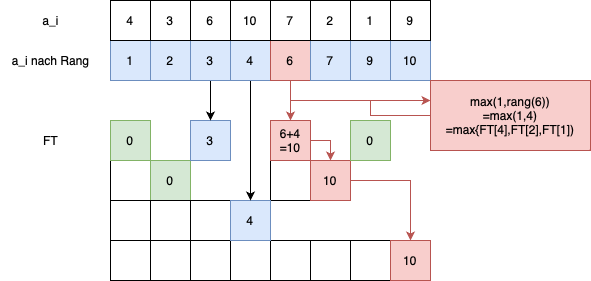
\includegraphics[scale=0.7]{./Pictures/FTexample.png}
\end{center}

Um die HIS zu rekonstruieren, wird ein $nodes$ Array benötigt, welche den neu eingetragenen Wert im FT an der Stelle $i$ (nicht $rang(a_i)$!) abspeichert. Wenn man dann von $n$ bis $1$ ($\sim$ rückwärts) durch $nodes$ läuft und $max(1,n)$ im FT findet, hat man das $a_i$ auf welches die HIS endet. Zieht man dieses vom Wert in $nodes$ ab, erhält man den nächsten Wert, der von der aktuellen Position aus gesucht wird. Durch eine einfache Anpassung, kann man auch bei mehreren Einträgen in $nodes$ mit dem gleichen Wert erkennen, welchen man nehmen muss. Dies sei dem Leser überlassen.

\begin{lstlisting}[mathescape]
res = max(1,FT.length);
for(i=FT.length;i$\geq 0$;i--){
	if(nodes[i]==res){
		print($a_i$);
		res-=$a_i$;
	}
}
\end{lstlisting}

